\documentclass{standalone}
\usepackage{tikz}
\begin{document}
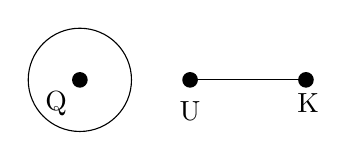
\begin{tikzpicture}
  \draw (0,0) node[circle,fill,inner sep=2pt] (Q) {};
  \draw (2.8713,0) node[circle,fill,inner sep=2pt] (K) {};
  \draw (1.4,0) node[circle,fill,inner sep=2pt] (U) {};
  \draw (U) -- (K);
  \draw (0,0) circle (0.6557cm);
  \node at (-0.3,-0.3) {Q};
  \node at (1.4,-0.4) {U};
  \node at (2.9,-0.3) {K};
\end{tikzpicture}
\end{document}